%% LyX 2.3.6.2 created this file.  For more info, see http://www.lyx.org/.
%% Do not edit unless you really know what you are doing.
\documentclass[english]{article}
\usepackage[T1]{fontenc}
\usepackage{geometry}
\geometry{verbose,tmargin=1in,bmargin=1in,lmargin=1in,rmargin=1in}
\usepackage{float}
\usepackage{amsmath}
\PassOptionsToPackage{normalem}{ulem}
\usepackage{ulem}
\usepackage{babel}
\usepackage[toc, page]{appendix}
\usepackage{float}
\usepackage{booktabs}
\usepackage{caption, subcaption}
\usepackage{graphicx}

\DeclareMathOperator{\dif}{d\!}

\begin{document}

\subsection*{A Model With Clean and Dirty Capital Stocks and and R\&D in Green Innovation-}

Assume there are two capital sectors, each with AK production technology
($Y_{i}=A_{i}K_{i},\,i\ =d, g)$ and each with its own capital stock
that evolves with quadratic adjustments costs and Brownian shocks
as follows:

\begin{align*}
\dif K_{d}/K_{d} & =[\alpha_{d}+i_{d}-\frac{\phi_{d}}{2}i_{d}^{2}]\dif t+\sigma_{d}\dif W\\
\dif K_{g}/K_{g} & =[\alpha_{g}+i_{g}-\frac{\phi_{g}}{2}i_{g}^{2}]\dif t+\sigma_{g}\dif W
\end{align*}


We also assume there is R\&D investment that leads to an increased arrival rate of a one time jump in Sector 2 productivity. The arrival rate is denoted as  t and evolves as follows

\begin{align*}
\dif \lambda_{t} / \lambda_t & =( \varphi  i_\lambda - \alpha_\lambda) \dif t+\sigma_{\lambda}\dif W
\end{align*}


The key di erence between the sectors is that production from Sector 1 generates emissions. As a result,the evolution of atmospheric temperature is give by the Matthews Approximation, so that temperature $Y_t$ and cumulative carbon emissions are given by

\begin{align*}
	\dif Y_t = E_t ( \beta_f \dif t + \varsigma \dif W)
\end{align*}

where  $\beta_f$ is the Matthews parameter and  $\eta$  is the scaling factor converting Sector $d$ output $ A_dK_d$ into emissions such that 
$$
E_t =  \eta A_dK_d
$$
Output can be used in for consumption, investment in either capital stock, or for R\&D into improving the productivity of Sector g :

\begin{align*}
C = A_dK_d - i_dK_d + A_gK_g - i_gK_g  - i_\lambda \lambda 	
\end{align*}
 

We assume exponential-quadratic damages to preferences so that our utility is augmented when accounting for climate damages. Flow utility is a log function over consumption, assuming perfect substitutability over output from the two sectors so that

\[
U(C)=\delta \log(A_dK_d - i_dK_d + A_gK_g - i_gK_g  - i_\lambda \lambda 	) -\delta \log N_{t}
\]

where the $\log N_{t}$ follows from BBH2 as
\begin{align*}
\log N_{t} & =\Gamma(Y)\\
\Gamma(y) & =\gamma_{1}y+\frac{\gamma_{2}}{2}y^{2}+\frac{\gamma_{3}}{2}\mathbf{1}_{y\ge\bar{y}}(y-\bar{y})^{2}
\end{align*}



Taking these pieces together we get the HJB equation

\begin{align*}
\delta V(K_{d},K_{g},\lambda,Y,\log N ) & =\max_{i_{g},i_{d}, i_{\lambda}}\delta \log(A_dK_d - i_dK_d + A_gK_g - i_gK_g  - i_\lambda \lambda ) -\delta \log N\\
 & +\{\alpha_{d}+i_{d}-\frac{\phi_{d}}{2}i_{d}^{2}\}V_{d}K_{d}+\{\alpha_{g}+i_{g}-\frac{\phi_{g}}{2}i_{g}^{2}\}V_{g}K_{g}+\frac{\sigma_{d}^{2}K_{d}^{2}}{2}V_{dd}+\frac{\sigma_{g}^{2}K_{g}^{2}}{2}V_{gg}\\
 & +\beta_{f}E_{d}V_{Y}+\frac{1}{2}\varsigma^{2}E_{d}^{2}V_{YY}+[\{\gamma_{1}+\gamma_{2}Y_{t}\}\beta_{f}E_{d}+\frac{\gamma_2}{2} \varsigma^{2}E_{d}^{2}]V_{\log N}+\frac{\varsigma^{2}E_{d}^{2}}{2}V_{\log N\log N}\\
 & +(\varphi i_{\lambda} - \alpha_\lambda)\lambda V_{\lambda}+\frac{(\sigma_{\lambda } \lambda)^{2}}{2}V_{\lambda \lambda}+\lambda  \left( V (K_d, K_g, \lambda, Y, \log N; A_g') - V (K_d, K_g, \lambda, Y, \log N; A_g) \right)
\end{align*}

The FOC for investment and R\&D are given by

\begin{align*}
0  =& -  \delta (A_dK_d - i_dK_d + A_gK_g - i_gK_g  - i_\lambda \lambda)^{-1} + (1 - \phi_d i_d) V_d\\
0 =& - \delta (A_dK_d - i_dK_d + A_gK_g - i_gK_g  - i_\lambda \lambda)^{-1} + (1 - \phi_d i_d) V_d\\
0 =&  - \delta (A_dK_d - i_dK_d + A_gK_g - i_gK_g  - i_\lambda \lambda)^{-1} + \varphi V_{\lambda}
\end{align*}


Using the fact that $\varphi V_{\lambda} = \delta (A_dK_d - i_dK_d + A_gK_g - i_gK_g  - i_\lambda \lambda)^{-1}$, we can simplify to

\begin{align*}
	i_d =&  \frac{1}{\phi_d} - \frac{\varphi}{\phi_d}\frac{V_\lambda}{V_d} \\
	i_g =& \frac{1}{\phi_g} - \frac{\varphi}{\phi_g}\frac{V_\lambda}{V_g}\\
	i_\lambda =&  \frac{1}{\lambda} \left( (A_d - (\frac{1}{\phi_d} - \frac{\varphi}{\phi_d}\frac{V_\lambda}{V_d}) ) K_d + (A_g - (\frac{1}{\phi_g} - \frac{\varphi}{\phi_g}\frac{V_\lambda}{V_g}) ) K_g - \frac{\delta}{\varphi V_\lambda} \right)
\end{align*}


We can analytically simplify out $\log Nt$ to get a simpli ed HJB

\begin{align*}
\delta v(K_{d},K_{g}, \lambda,Y) & =\max_{i_{g},i_{d}, i_\lambda }\delta \log(A_dK_d - i_dK_d + A_gK_g - i_gK_g  - i_\lambda \lambda ) \\
 & +\{\alpha_{d}+i_{d}-\frac{\phi_{d}}{2}i_{d}^{2}\}v_{d}K_{d}+\{\alpha_{g}+i_{g}-\frac{\phi_{g}}{2}i_{g}^{2}\}v_{g}K_{g}+\frac{\sigma_{d}^{2}K_{d}^{2}}{2}v_{dd}+\frac{\sigma_{g}^{2}K_{g}^{2}}{2}v_{gg}\\
 & +\beta_{f}E_{d}v_{Y}+\frac{1}{2}\varsigma^{2}E_{d}^{2}v{}_{YY} - [\{\gamma_{1}+\gamma_{2}Y_{t}\}\beta_{f}E_{d}+\frac{\gamma_2}{2}\varsigma^{2}E_{d}^{2}]\\
 & +(-\alpha_{\lambda}  + \varphi i_\lambda) \lambda v_{\lambda}+\frac{(\sigma_{\lambda} \lambda)^2}{2}v_{\lambda\lambda}+\lambda \left( v (K_d, K_g, \lambda, Y; A_g') - v (K_d, K_g, \lambda, Y; A_g) \right)
\end{align*}

FOC

\begin{align*}
	i_d =&  \frac{1}{\phi_d} - \frac{\varphi}{\phi_d}\frac{v_\lambda}{v_d} \\
	i_g =& \frac{1}{\phi_g} - \frac{\varphi}{\phi_g}\frac{v_\lambda}{v_g}\\
	i_\lambda =&  \frac{1}{\lambda} \left( (A_d - (\frac{1}{\phi_d} - \frac{\varphi}{\phi_d}\frac{v_\lambda}{v_d}) ) K_d + (A_g - (\frac{1}{\phi_g} - \frac{\varphi}{\phi_g}\frac{v_\lambda}{v_g}) ) K_g - \frac{\delta}{\varphi v_\lambda} \right)
\end{align*}

From this we can layer on different forms of uncertainty.

\section{Post jump}

Replace $E_d $ with $\eta A_d K_d$.
We solve post jump HJB:

\begin{align*}
	\delta v(K_{d}, K_{g}, Y; A_g') & =\max_{i_{g},i_{d} }\delta \log(A_dK_d - i_dK_d + A_g'K_g - i_gK_g  ) \\
	& +\{\alpha_{d}+i_{d}-\frac{\phi_{d}}{2}i_{d}^{2}\}v_{d}K_{d}+\{\alpha_{g}+i_{g}-\frac{\phi_{g}}{2}i_{g}^{2}\}v_{g}K_{g}+\frac{\sigma_{d}^{2}K_{d}^{2}}{2}v_{dd}+\frac{\sigma_{g}^{2}K_{g}^{2}}{2}v_{gg}\\
	& +\beta_{f} (\eta A_d K_d )v_{Y}+\frac{1}{2}\varsigma^{2}(\eta A_d  K_d)^{2}v{}_{YY} - [\{\gamma_{1}+\gamma_{2}Y_{t}\}\beta_{f}(\eta A_d K_d)+\frac{\gamma_2}{2}\varsigma^{2}(\eta A_d K_d)^{2}]
\end{align*}

denote
\begin{align*}
	mc =  \delta (A_dK_d - i_dK_d + A_g'K_g - i_gK_g  )^{-1}
\end{align*}

FOC

\begin{align*}
	i_d =&  \frac{1}{\phi_d} - \frac{mc}{\phi_d v_d} \\
	i_g =& \frac{1}{\phi_g} - \frac{mc}{\phi_g v_g}
\end{align*}

\begin{gather*}
	X = [\log K, L, Y]',  \quad \log K = \log(K_d + K_g), \quad  L = \log K_g - \log K_d\\
	R = \frac{K_g}{K_d + K_g} = \frac{\exp(L)}{1 + \exp(L)} 
\end{gather*}

\begin{align*}
	\dif (K_{d} + K_g) =& \left([\alpha_{d}+i_{d}-\frac{\phi_{d}}{2}i_{d}^{2}] K_d + [\alpha_{g}+i_{g}-\frac{\phi_{g}}{2}i_{g}^{2}] K_g \right)\dif t+\left(\sigma_{d}K_d + \sigma_g K_g \right)\dif W\\
		\dif K / K =&  \left([\alpha_{d}+i_{d}-\frac{\phi_{d}}{2}i_{d}^{2}] (1 - R) + [\alpha_{g}+i_{g}-\frac{\phi_{g}}{2}i_{g}^{2}] R \right) \dif t+\left(\sigma_{d}(1 - R)+ \sigma_g R \right)\dif W \\
		\dif \log K =& \left([\alpha_{d}+i_{d}-\frac{\phi_{d}}{2}i_{d}^{2}] (1 - R) + [\alpha_{g}+i_{g}-\frac{\phi_{g}}{2}i_{g}^{2}] R - \frac{\mid\sigma_{d}(1 - R)+ \sigma_g R \mid
		^2}{2} \right) \dif t\\
		 &+\left(\sigma_{d}(1 - R)+ \sigma_g R \right)\dif W
\end{align*}

\begin{align*}
	\dif L = \dif (\log K_g - \log K_d) = \left( (\alpha_g + i_d  - \frac{\phi_{g}}{2}i_g^2) -  (\alpha + i_d - \frac{\phi_d}{2} i_d^2)\right) \dif t  + (\sigma_g - \sigma_d) \dif W
\end{align*}

\begin{align*}
 	\dif Y = \eta A_d   (1 - R) K ( \beta_f \dif t +  \varsigma \dif W)
\end{align*}

\begin{align*}
	\delta v(\log K, L,  Y; A_g') & =\max_{i_{g},i_{d} }\delta \log((A_d - i_d) (1 - R) + (A_g' - i_g)R  ) + \delta \log K \\
	& +\left(\{\alpha_{d}+i_{d}-\frac{\phi_{d}}{2}i_{d}^{2}\} (1 - R)+\{\alpha_{g}+i_{g}-\frac{\phi_{g}}{2}i_{g}^{2}\} R  - \frac{\mid\sigma_{d}(1 - R)+ \sigma_g R \mid
		^2}{2}\right) v_k  \\
	&+\frac{\mid \sigma_{d} (1 - R) + \sigma_g R\mid^2}{2}v_{kk}\\
	&+ \left( (\alpha_g + i_g  - \frac{\phi_{g}}{2}i_g^2) -  (\alpha + i_d - \frac{\phi_d}{2} i_d^2)\right) v_l \\
	& +\beta_{f} (\eta A_d (1 - R) K )v_{Y}+\frac{1}{2}\varsigma^{2}(\eta A_d  (1 - R) K)^{2}v{}_{YY} \\
	&- [\{\gamma_{1}+\gamma_{2}Y_{t}\}\beta_{f}(\eta A_d(1 - R)K)+\frac{\gamma_2}{2}\varsigma^{2}(\eta A_d (1 - R) K)^{2}]
\end{align*}


\begin{align*}
	\delta v(\log K, R,  Y; A_g') & =\max_{i_{g},i_{d} }\delta \log((A_d - i_d) (1 - R) + (A_g' - i_g)R  ) + \delta \log K \\
	& +\left(\{\alpha_{d}+i_{d}-\frac{\phi_{d}}{2}i_{d}^{2}\} (1 - R)+\{\alpha_{g}+i_{g}-\frac{\phi_{g}}{2}i_{g}^{2}\} R  - \frac{\mid\sigma_{d}(1 - R)+ \sigma_g R \mid
		^2}{2}\right) v_k  \\
	&+\frac{\mid \sigma_{d} (1 - R) + \sigma_g R\mid^2}{2}v_{kk}\\
	&+ \left( (\alpha_g + i_g  - \frac{\phi_{g}}{2}i_g^2) -  (\alpha + i_d - \frac{\phi_d}{2} i_d^2)\right) \left[ R(1 - R)\right] v_r \\
	& +\beta_{f} (\eta A_d (1 - R) K )v_{Y}+\frac{1}{2}\varsigma^{2}(\eta A_d  (1 - R) K)^{2}v{}_{YY} \\
	&- [\{\gamma_{1}+\gamma_{2}Y_{t}\}\beta_{f}(\eta A_d(1 - R)K)+\frac{\gamma_2}{2}\varsigma^{2}(\eta A_d (1 - R) K)^{2}]
\end{align*}

FOC
\begin{align*}
	mc = \delta ((A_d - i_d) (1 - R) + (A_g' - i_g)R )^{-1}
\end{align*}

\begin{align*}
	mc  =& (1 - \phi_d i_d) \left(( v_k - R v_r \right) &\Rightarrow i_d &= \frac{1}{\phi_d} \left[ 1 - \frac{ mc}{v_k  - R v_r }\right] \\
	mc =& (1 - \phi_g i_g) \left(v_k + (1 - R) v_l\right) &\Rightarrow i_g &= \frac{1}{\phi_g}\left[1 - \frac{ mc}{v_k + (1 - R) v_r}\right]
\end{align*}


\subsection{tests}

\subsubsection{Preliminary results: try $i_d = i_g = 0$, no optimization}

\begin{figure}[H]
	\centering
	\begin{subfigure}{0.45\textwidth}
		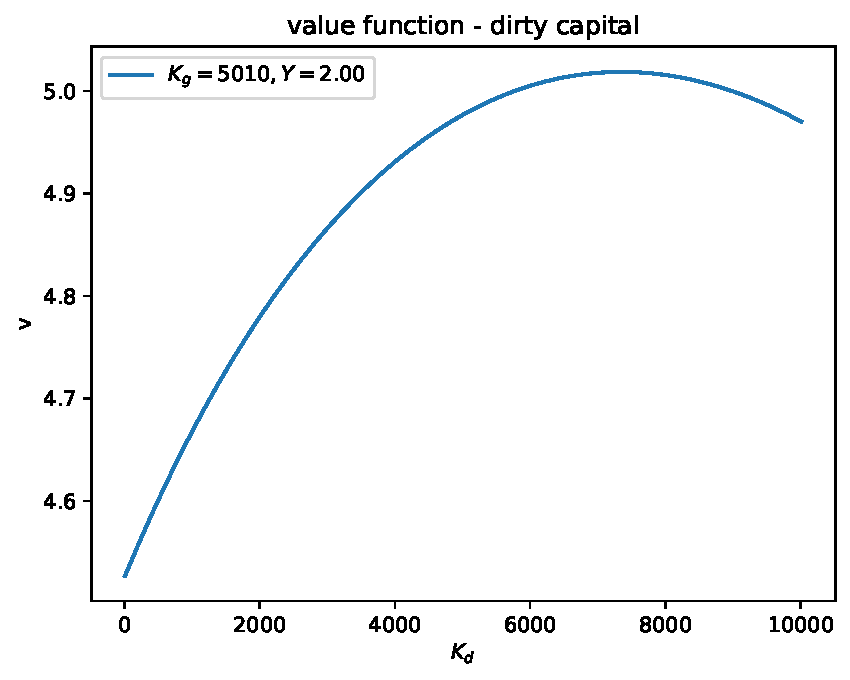
\includegraphics[width=\textwidth]{../figures/v-Kd.pdf}
	\end{subfigure}
\hspace{\fill}
\begin{subfigure}{0.45\textwidth}
	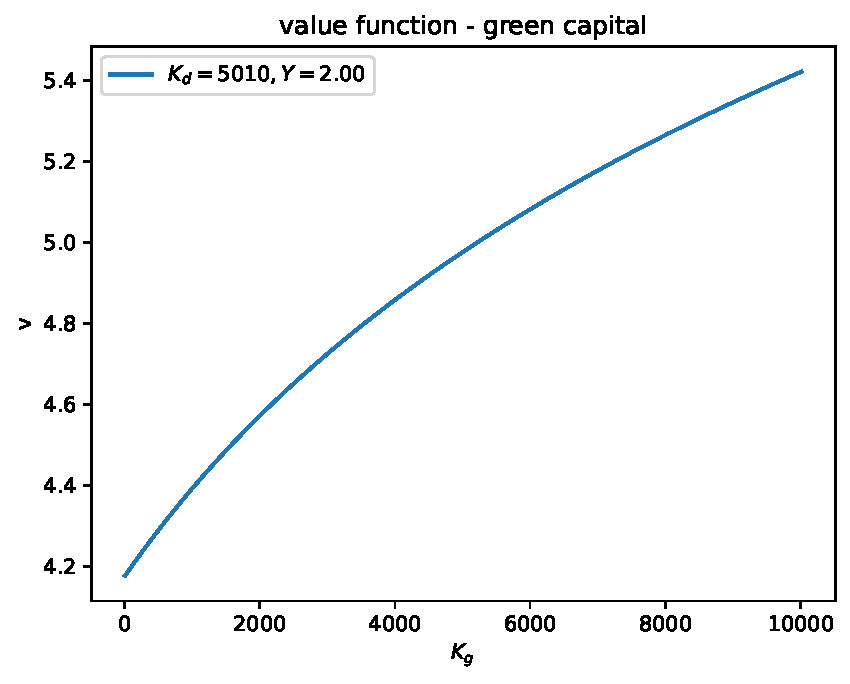
\includegraphics[width=\textwidth]{../figures/v-Kg.pdf}
\end{subfigure}
\begin{subfigure}{0.45\textwidth}
	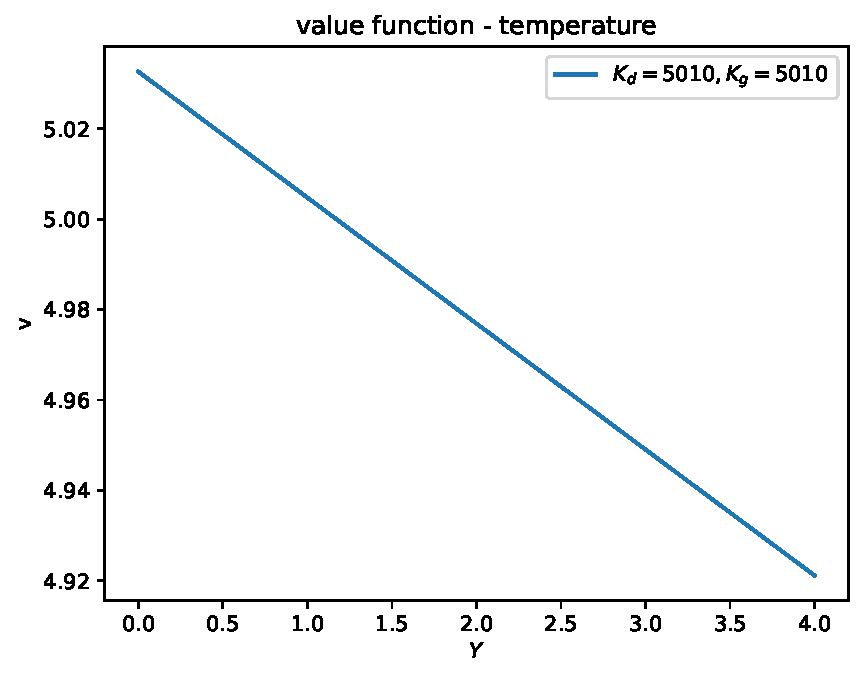
\includegraphics[width=\textwidth]{../figures/v-Y.pdf}
\end{subfigure}
\caption{Results for value function, $i_d= 0, i_g=0$}
\end{figure}

\subsubsection{steady state}
try set
\begin{align*}
	\alpha_d + i_d - \frac{\phi_d}{2} i_d^2 = 0 \Rightarrow i_d^* = 0.022\\
	\alpha_g + i_g - \frac{\phi_g}{2} i_g^2 = 0 \Rightarrow i_g^* = 0.022
\end{align*}



\begin{figure}[H]
	\centering
	\begin{subfigure}{0.4\textwidth}
		\includegraphics[width=\textwidth]{../figures/v-Kd-stat.pdf}
	\end{subfigure}
	\hspace{\fill}
	\begin{subfigure}{0.4\textwidth}
		\includegraphics[width=\textwidth]{../figures/v-Kg-stat.pdf}
	\end{subfigure}
	\begin{subfigure}{0.4\textwidth}
		\includegraphics[width=\textwidth]{../figures/v-Y-stat.pdf}
	\end{subfigure}
	\caption{Results for value function,  $i_d^* = 0.022, i_g^*=0.022$}
\end{figure}

%
%\begin{figure}[H]
%	\centering
%	\begin{subfigure}{0.4\textwidth}
%		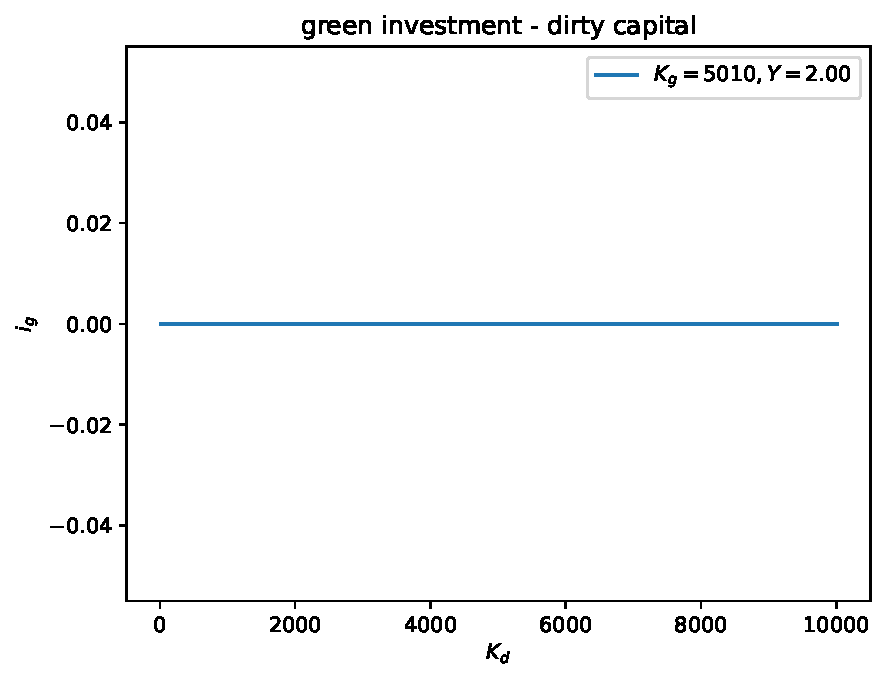
\includegraphics[width=\textwidth]{../figures/ig-Kd.pdf}
%	\end{subfigure}
%	\hspace{\fill}
%	\begin{subfigure}{0.4\textwidth}
%		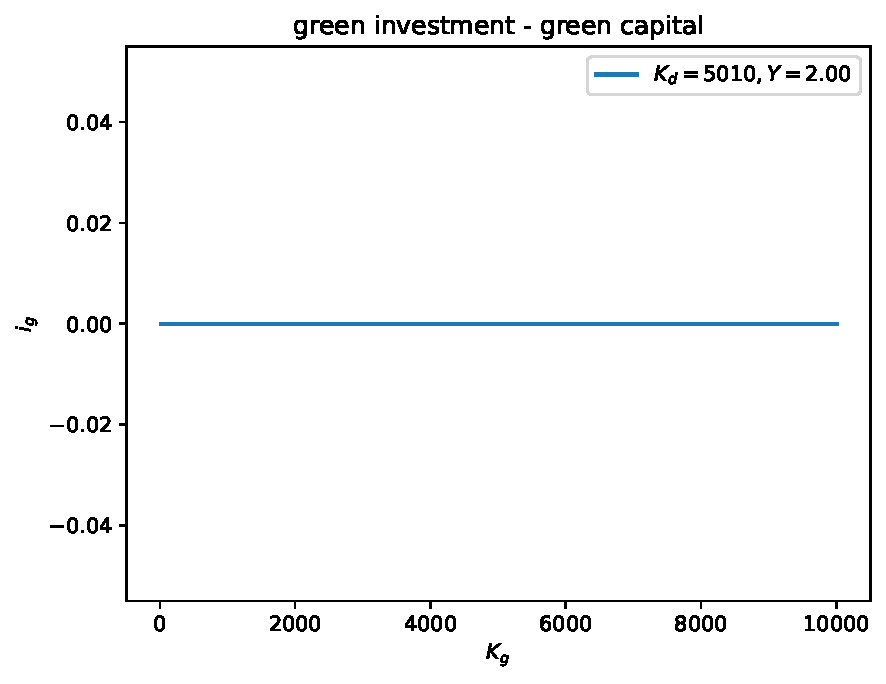
\includegraphics[width=\textwidth]{../figures/ig-Kg.pdf}
%	\end{subfigure}
%	\begin{subfigure}{0.4\textwidth}
%		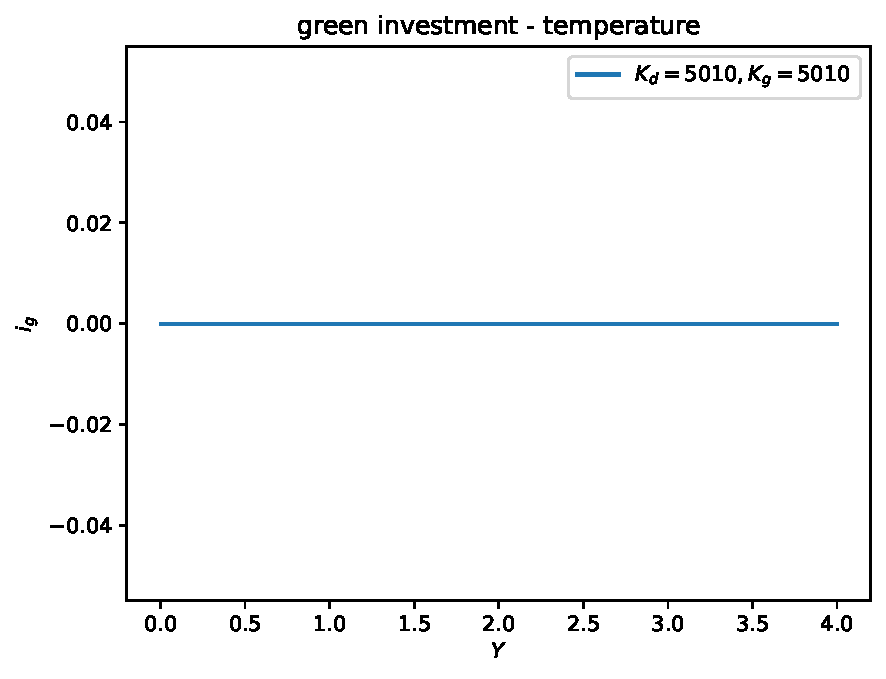
\includegraphics[width=\textwidth]{../figures/ig-Y.pdf}
%	\end{subfigure}
%	\caption{Results for green investment}
%\end{figure}

\section{Pre jump}

\appendix
\section{State variables}
Capital:
\begin{align*}
	K_d \in& [0, 10, 000]\\
	K_g \in& [0, 10,000]\\
	\lambda \in& [0, 0.1]\\
	Y \in& [0, 4]
\end{align*}

\section{Parameters}

Economy
\begin{table}[H]
	\centering
	\begin{tabular}{ll}
		Parameters & values\\
		\toprule
		$\delta$ & 0.01\\
		$(\alpha_d, \phi_d, \sigma_d)$ & ( -0.02, 8, 0.016)\\
		$(\alpha_g, \phi_g, \sigma_g)$ & ( -0.02, 8, 0.016) \\
		$(\alpha_\lambda, \varphi, \sigma_\lambda)$ & (0, 0.1, 0.016)\\
		$A_d$ & 0.12\\
		$(A_g, A_g')$ & (0.10, 0.15)\\
		\bottomrule
	\end{tabular}
\end{table}


Temperature and damage
\begin{table}[H]
	\centering
	\begin{tabular}{ll}
		Parameters & values\\
		\toprule
		$\beta_f$ & 1.86 / 1000\\
		$\varsigma$ & 1.2 * 1.86 / 1000\\
		$\gamma_1$ &  0.00017675 \\
		$\gamma_2$ &   2 * 0.0022 \\
		$\gamma_3$ & 0\\
		$\bar{y}$ & 2\\
		\bottomrule
	\end{tabular}
\end{table}

$\eta$ are determined as follows:
\begin{itemize}
	\item Initial capital: $K_0 = 85 / 0.115 \approx 739$
	\item $K_{d, 0} = K_0 \times \frac{2}{3} \approx  493$
	\item Choose $\eta$ such that $10 = \eta \times 0.12 \times 493 \Rightarrow \eta \approx 0.17$
\end{itemize}

\end{document}
